\documentclass[a4paper]{jpconf}
\usepackage{graphicx}
\begin{document}
\title{Simulation of liquid cube fracture with SPH}

\author{M N Davydov}

\address{Lavrentyev Institute of Hydrodynamics of the Siberian Branch of the Russian Academy of Sciences, Novosibirsk, Russia}

\ead{davydov@hydro.nsc.ru}


\begin{abstract}
The dynamics of fracture of liquid cube with high-pressure cavity is studied numerically in a three-dimensional formulation using the Smoothed Particle Hydrodynamics method (SPH).  It is shown that the propogation of shock wave from growing cavity and reflection from the free side is due to relaxation of tensile stresses in the liquid volume and formation of quasistationary mass-velocity field which provides fracture of the fluid. 
\end{abstract}

\section{Introduction}

The problem of liquid breakdown in intense rarefaction waves is directly related to the
notion of strength, which does not have a precise and clear definition in the mechanics of liquids under dynamic
loading, unlike in solid mechanics~\cite{DavydovKedrinskii2008}. A typical examples of this process is the ejection fraction of magmatic melt from the channel of the volcano during the exposive eruption~\cite{Davydov2012a} or the formation of sultans out on the free surface at shallow underwater explosions.


Numerical methods based on finite differences are unable to solve such problems, therefore it is  required to use methods that can simulate of flows in the complex variable geometry region. In this paper, a model problem of an underwater explosion in the cube of pure (one-phase) liquid using the SPH method~\cite{Monaghan2005}  is considered.

\section{SPH method}

The smoothed particle hydrodynamics (SPH) method~\cite{Monaghan1992,Monaghan2005} is an effective meshless Lagrangian numerical
method used to calculate flow structures with an unknown free boundary, in particular, high-velocity processes in
media with the modeled object topology appreciably changed under intense dynamic loading.

In this method $N$ spherical particles are placed into the modeled physical space. Each particle has a
mass $m_i$, internal energy $e_i$, and velocity $\vec{v}_i$. The particles move in accordance with the laws of mechanics. If these
physical quantities are known at a certain time at all points $j = 1,\ldots{},N$ to which $N$ particles are placed, i.e., if
a certain function $f(r_j)$ is specified, then its value at an arbitrary point of the modeled space can be obtained by
means of discretization of the interpolation formula
\[ \left\langle f(r) \right\rangle = \int f(r') W(r-r', h) dr,\]
where $h$ is the smoothing radius and $W(r-r', h)$ is the smoothing function (kernel) for which the following conditions
should be satisfied:
\[ \int W(r,h) dr = 1, \qquad   \lim_{h \to 0} W(r,h)=\delta(r)\]
In this work we use the known definition of the kernel based on third-order piecewise-spline functions~\cite{Monaghan1992}.	

As the smoothing function $W$ is not equal to zero only in a certain (small) neighborhood of the point with the
coordinate $r$, the result of interpolation is affected only by those nodes that are located in the neighborhood of
smoothing of this point. Therefore, it is possible to avoid summation over all known values of the function and to
perform it only over the neighboring nodes (particles) located at distances smaller than $2h$.

It should be noted that the procedure of sampling of all particles in space has a quadratic order of complexity,
and it is next to impossible to implement it in practice. As the particles arbitrarily move in space and can freely
mix, the task of effective (time-efficient) searching for the neighboring particles is extremely important for the
SPH method. One possible approach to solving this problem is to divide the space into cells and to perform
summation only over particles in the neighboring cells. It should be noted that the mesh constructed for this
purpose is an auxiliary tool used for accelerating the process of searching for the neighboring particles rather than
for approximation; therefore, it does not affect the resultant solution, and the SPH method is still a meshless one.
	
	In the SPH method the gas dynamic equations have the form
	\[  \frac{\partial \rho_i}{\partial t} = - \rho_i \sum\limits_{j=1}^{N} \frac{m_j}{\rho_j} (v_j -  v_i) \nabla W(r_i - r_j,h)
\]
\[\frac{\partial v_i}{\partial t} = - \sum\limits_{j=1}^{N} m_j \left ( \frac{p_i}{\rho_i^2} + \frac{p_j}{\rho_j^2} \right) \nabla W(r_i-r_j,h).\]

We use the known definition of the liquid state equation:  
\[p= p_0 + \frac{\rho_0 c_0^2}{\gamma} \left[ \left( \frac{\rho}{\rho_0} \right)^{\gamma} - 1 \right],\]
where  $\gamma = 7.15$, $\rho_0$ and $p_0$ is a reference density and pressure, $c_0$ is a speed of sound (approximate 1500 m/s).

			
\section{Results of numerical simulations}


Initially, the liquid is a cube with sides of $1$~cm, located on the $XY$ plane, $OZ$ axis passes through the center of the cube. Inside the liquid, at a distance of $2.5$~mm from the top side of the cube, there is a spherical cavity radius of $1$~mm, the center of which is located on the axis $OZ$. The pressure in the cavity is $10000$~atm, the rest of the liquid is at atmospheric pressure $p_0$. 
Figure~\ref{P-Vel-1}--\ref{P-Vel-25} shows the distribution of pressure and particle velocities in the central section of the cube (the plane $y=0$).

\begin{figure}
\begin{center}
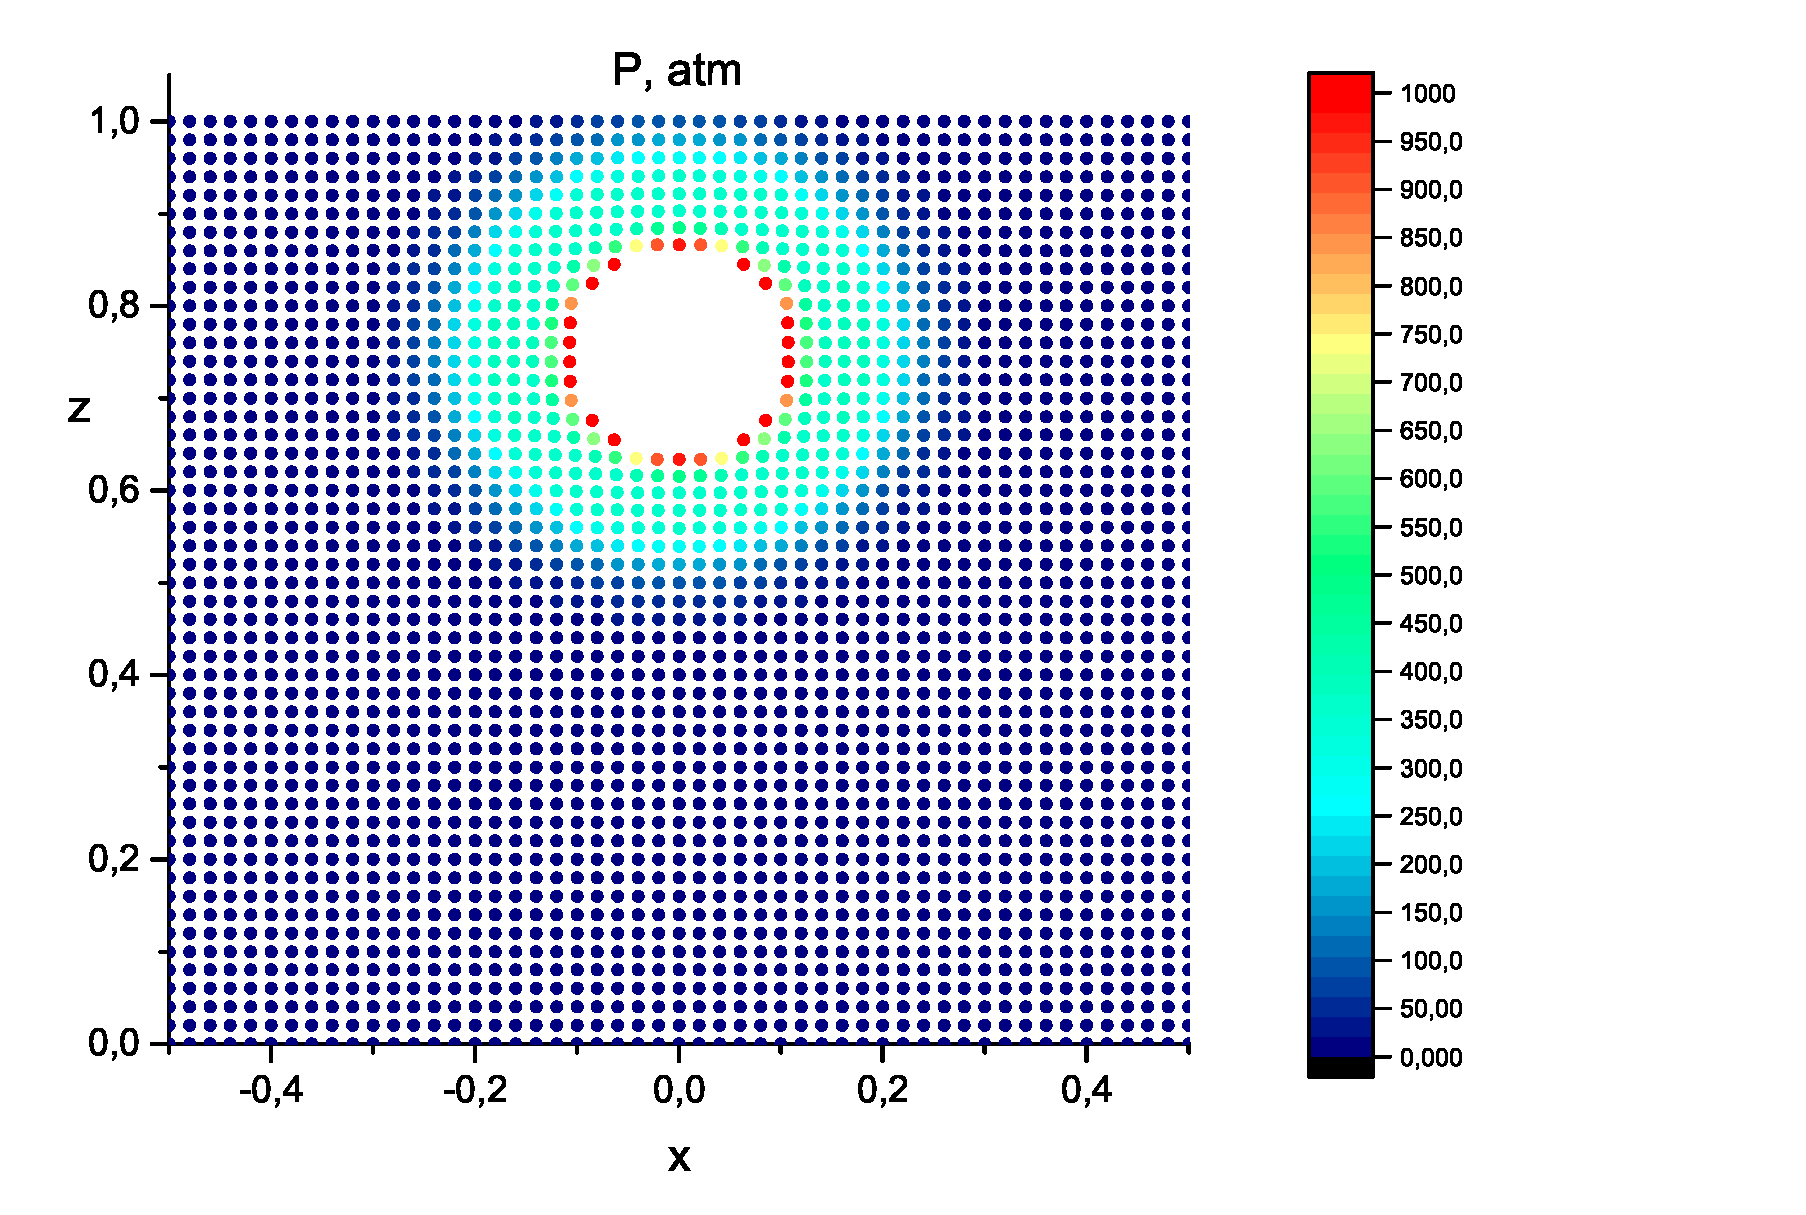
\includegraphics[width=0.6\textwidth]{P-1.eps}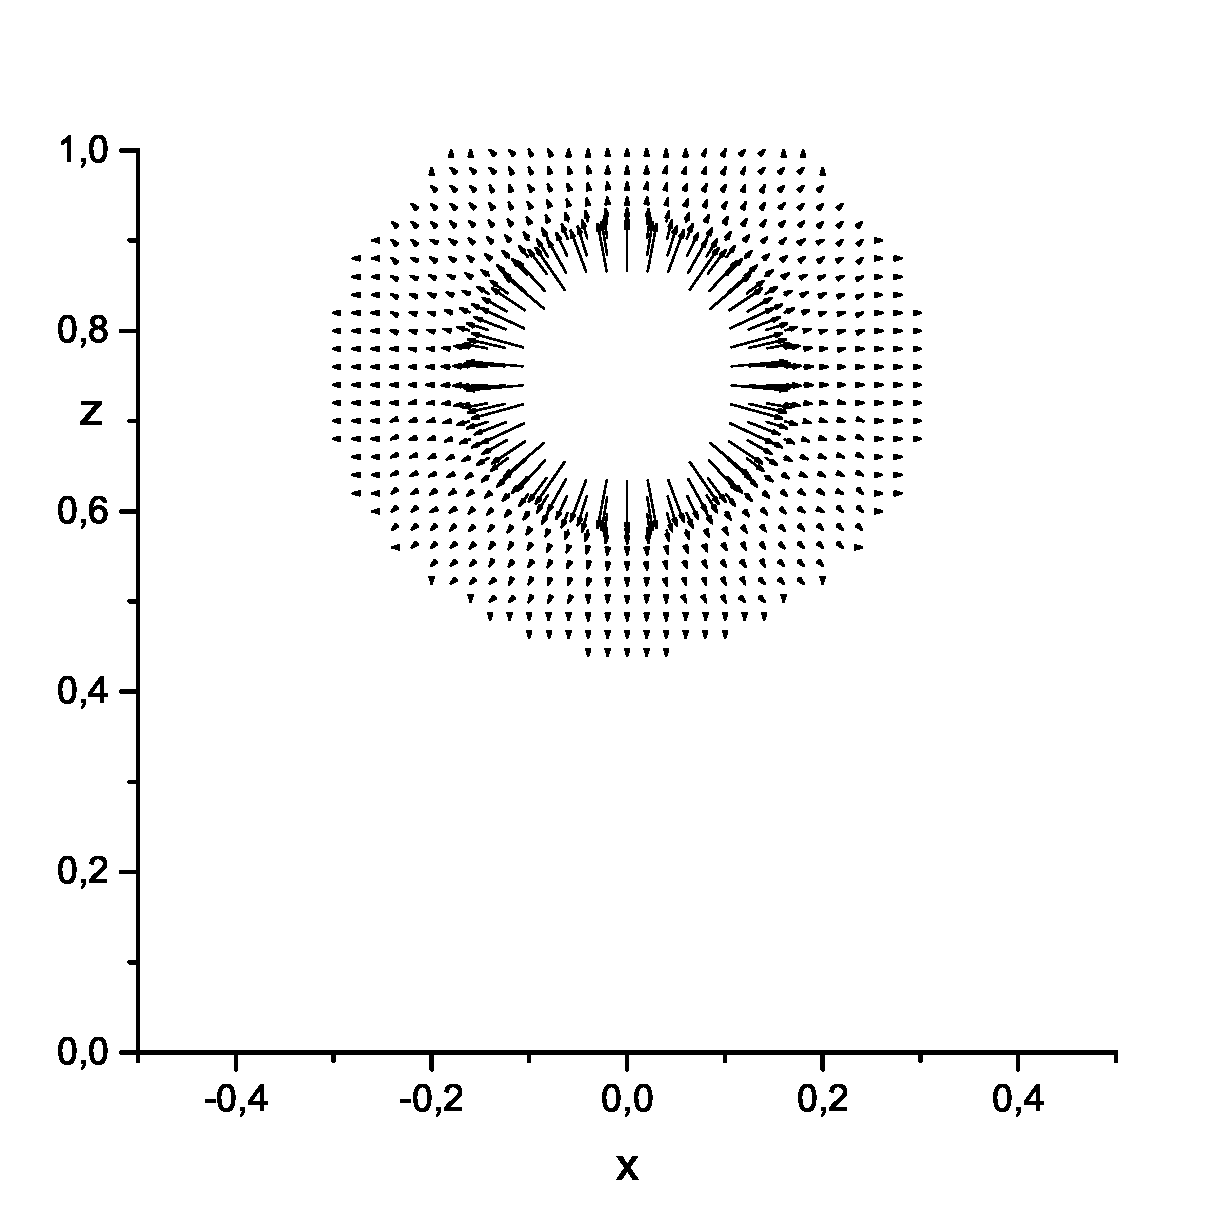
\includegraphics[width=0.4\textwidth]{Vel-1.eps}
\end{center}
\caption{\label{P-Vel-1} Distribution of pressure and particle velocities in the central section of the cube ($1$~$\mu$s)}
\end{figure}


The shock wave propagates from the high-pressure cavity. The amplitude of shock wave decreases as it propagates. 
Figure \ref{P-Vel-1} shows the begin of reflection the shock wave from the top of the cube at time $1$~$\mu$s. Near to the cavity layer of liquid starts to move. Only particles in which $\vec{v} \neq 0$ is painted on the figure. It is clearly seen that the velocity distribution is symmetric with respect to the cavity.
 
\begin{figure}
\begin{center}
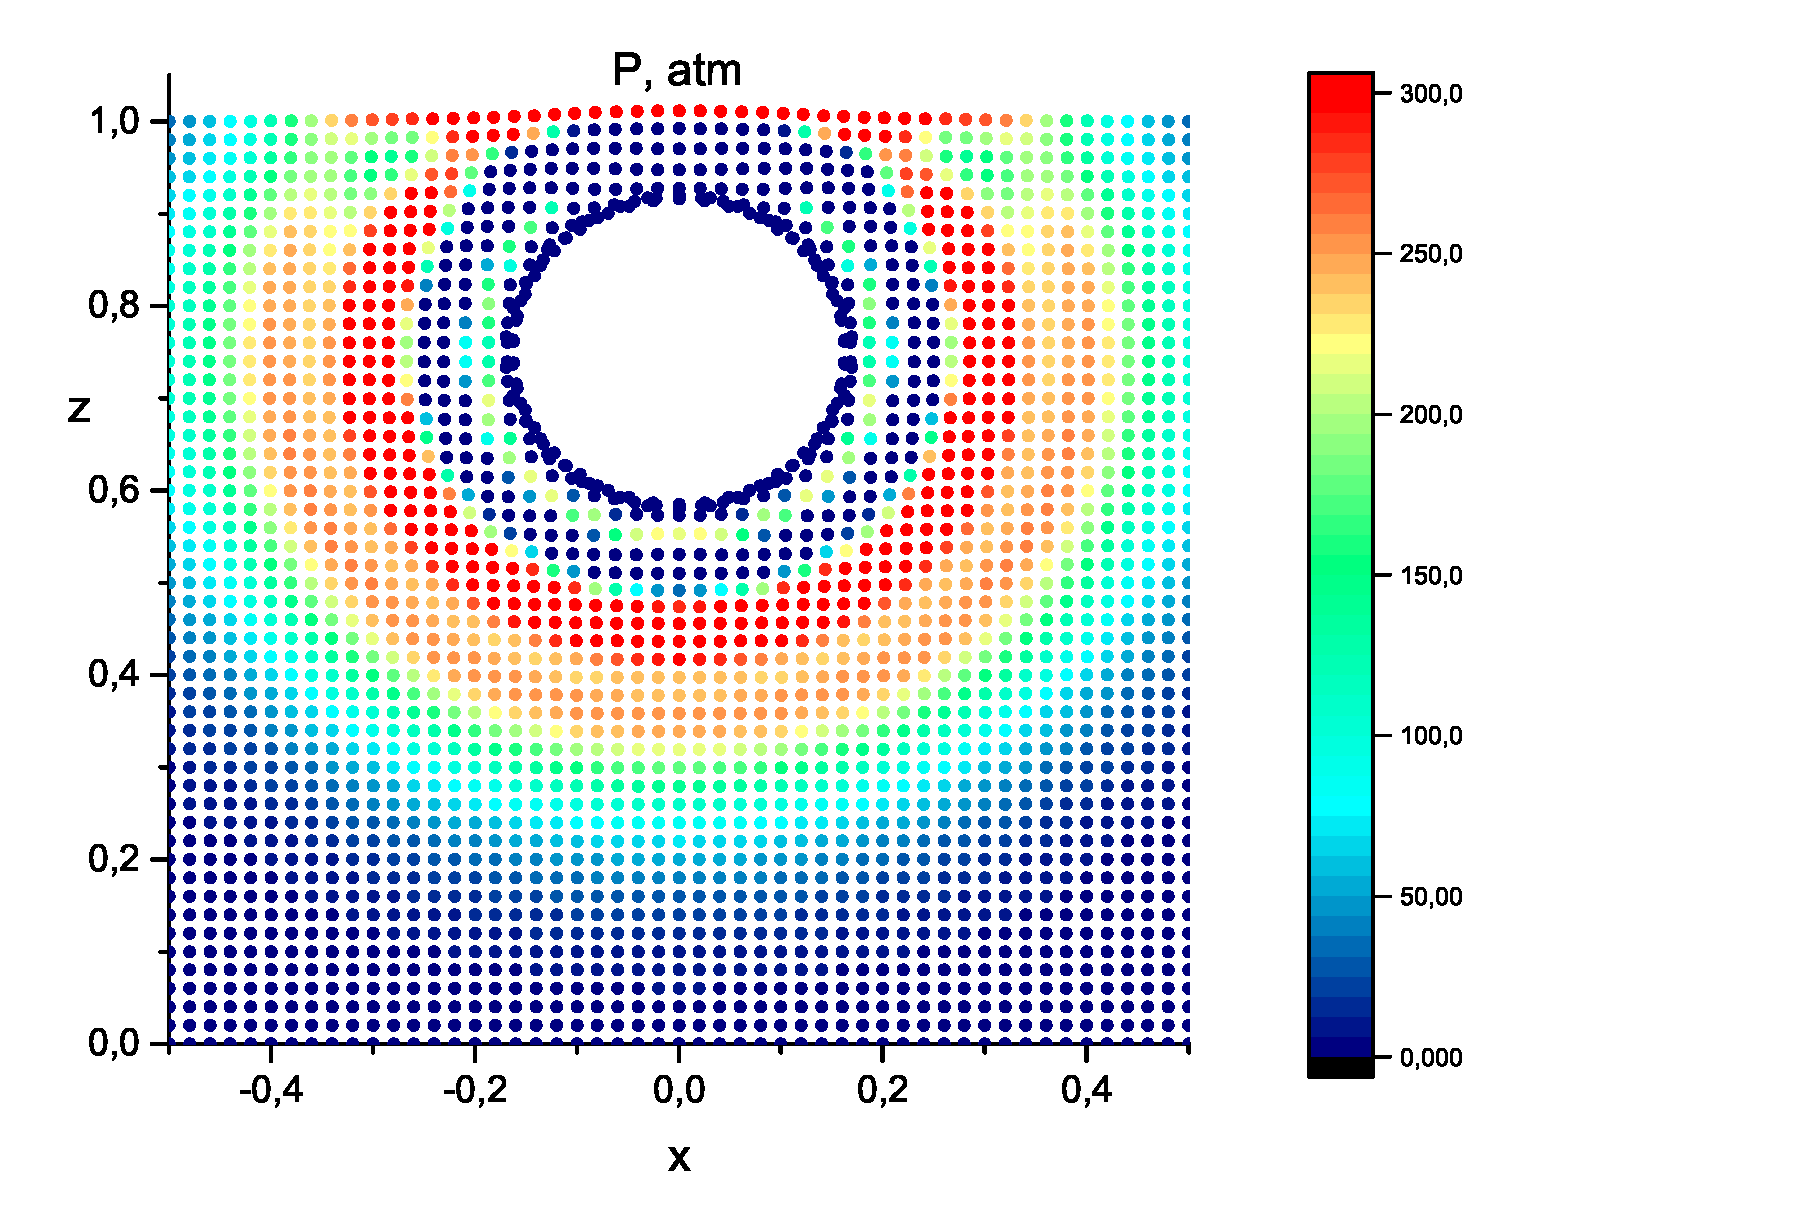
\includegraphics[width=0.6\textwidth]{P-5.eps}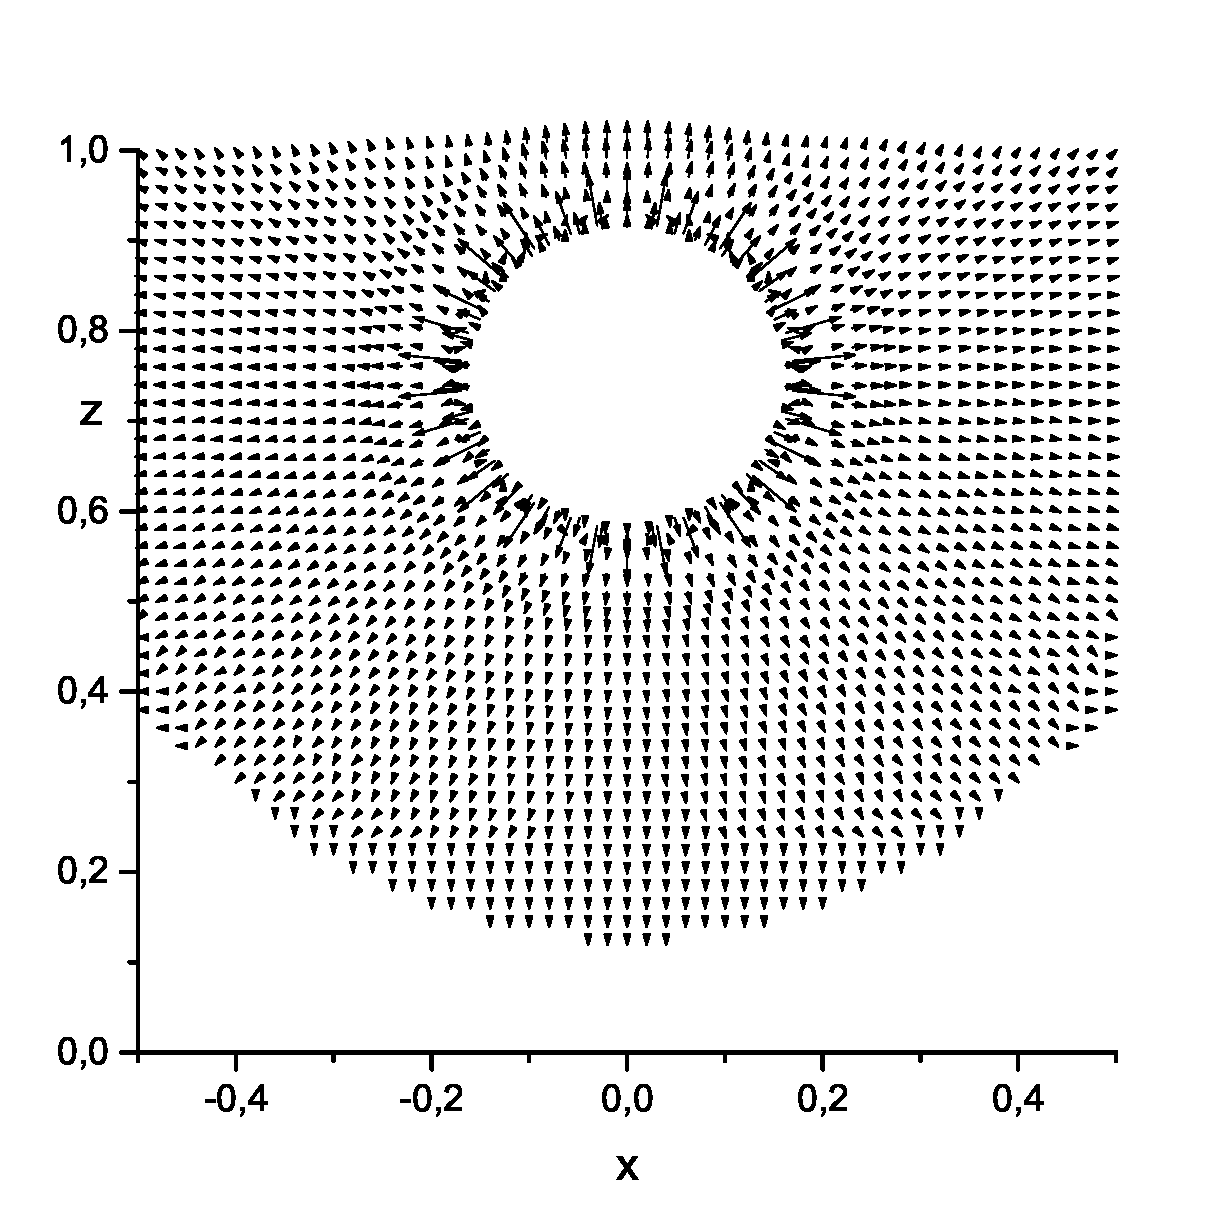
\includegraphics[width=0.4\textwidth]{Vel-5.eps}
\end{center}
\caption{\label{P-Vel-5} Distribution of pressure and particle velocities in the central section of the cube ($5$~$\mu$s)}
\end{figure}


Figure \ref{P-Vel-5} shows that the wave reaches the faces of the cube and is reflected from its borders, at first it occurs on the side face, then on the bottom. By this time, the upper bound is significantly deformed, curling up. 
Almost all particles are in motion, it is clear that the particles at the boundary of the cavity ``push'' other particles.

\begin{figure}
\begin{center}
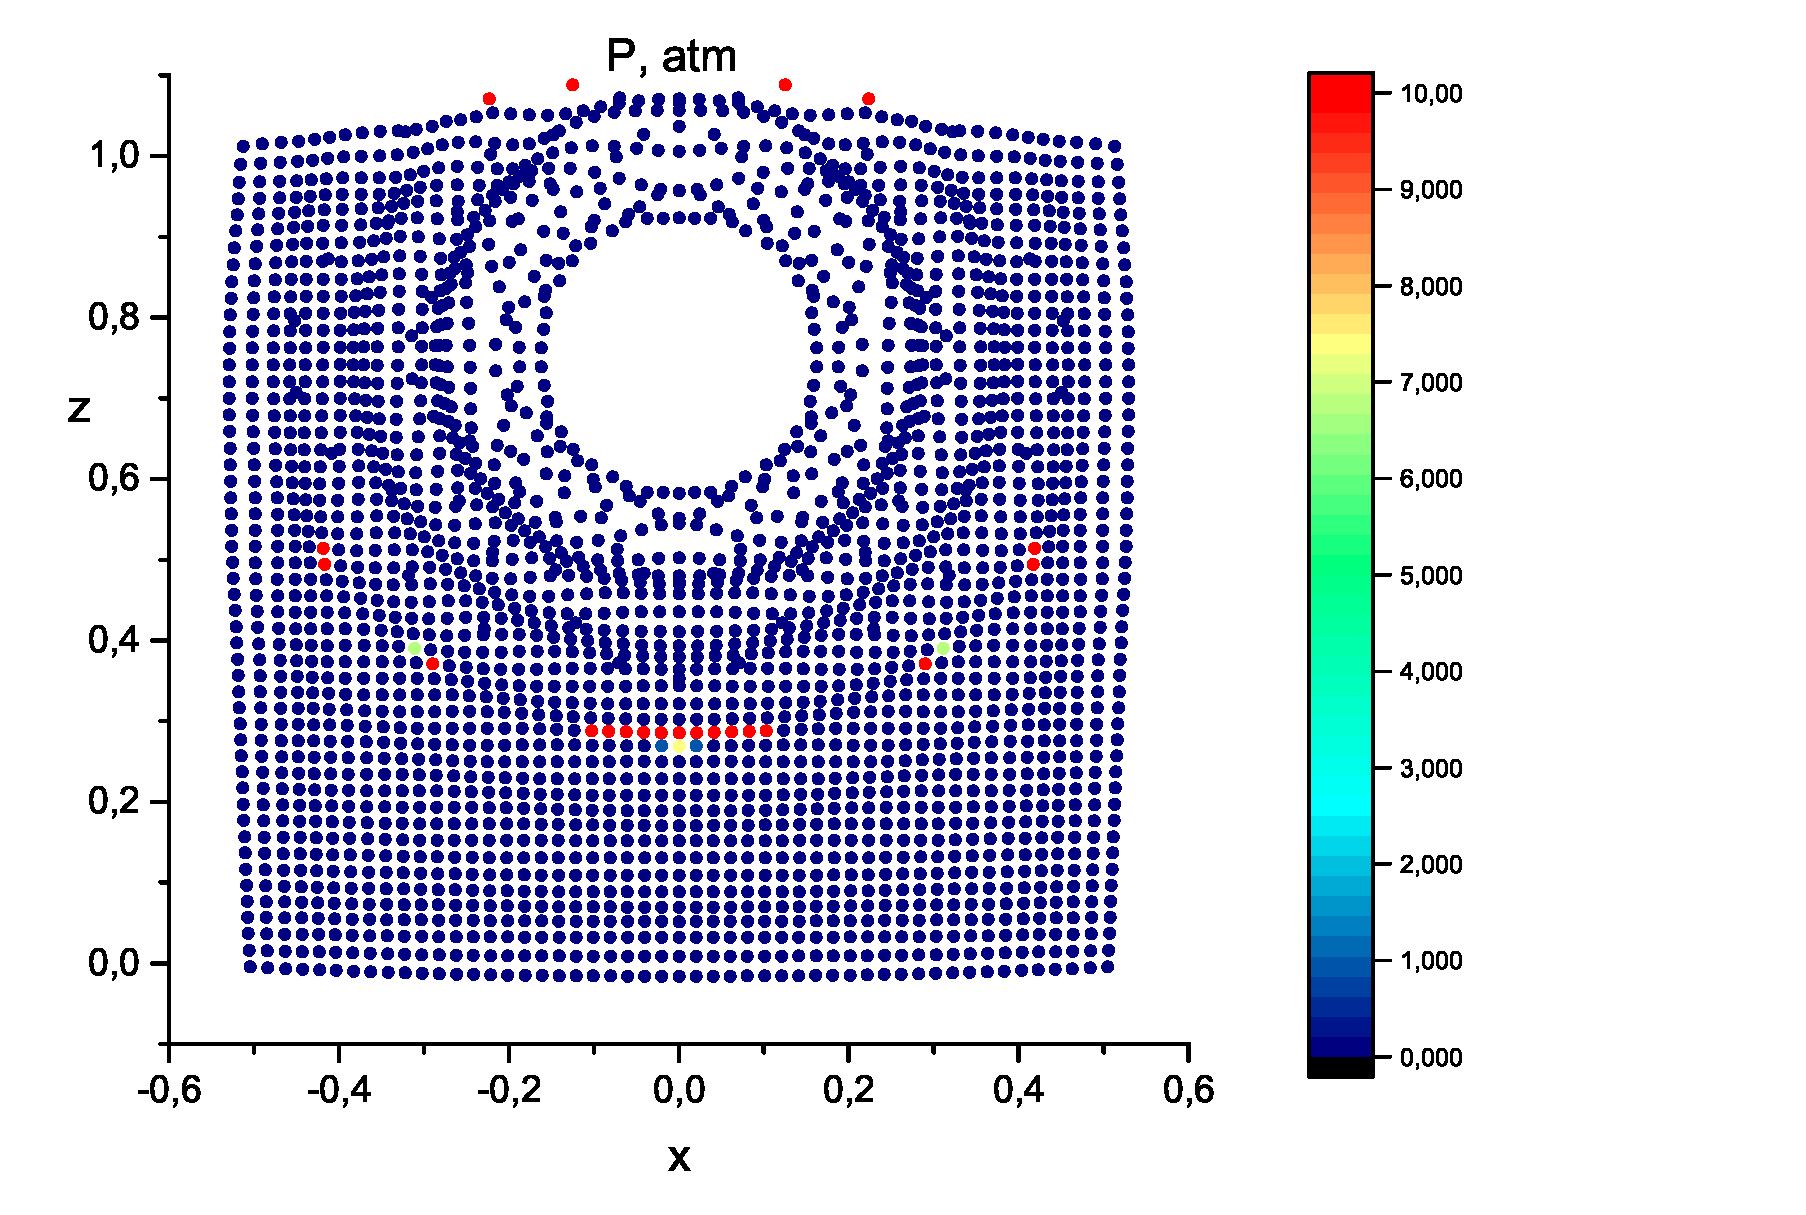
\includegraphics[width=0.6\textwidth]{P-25.eps}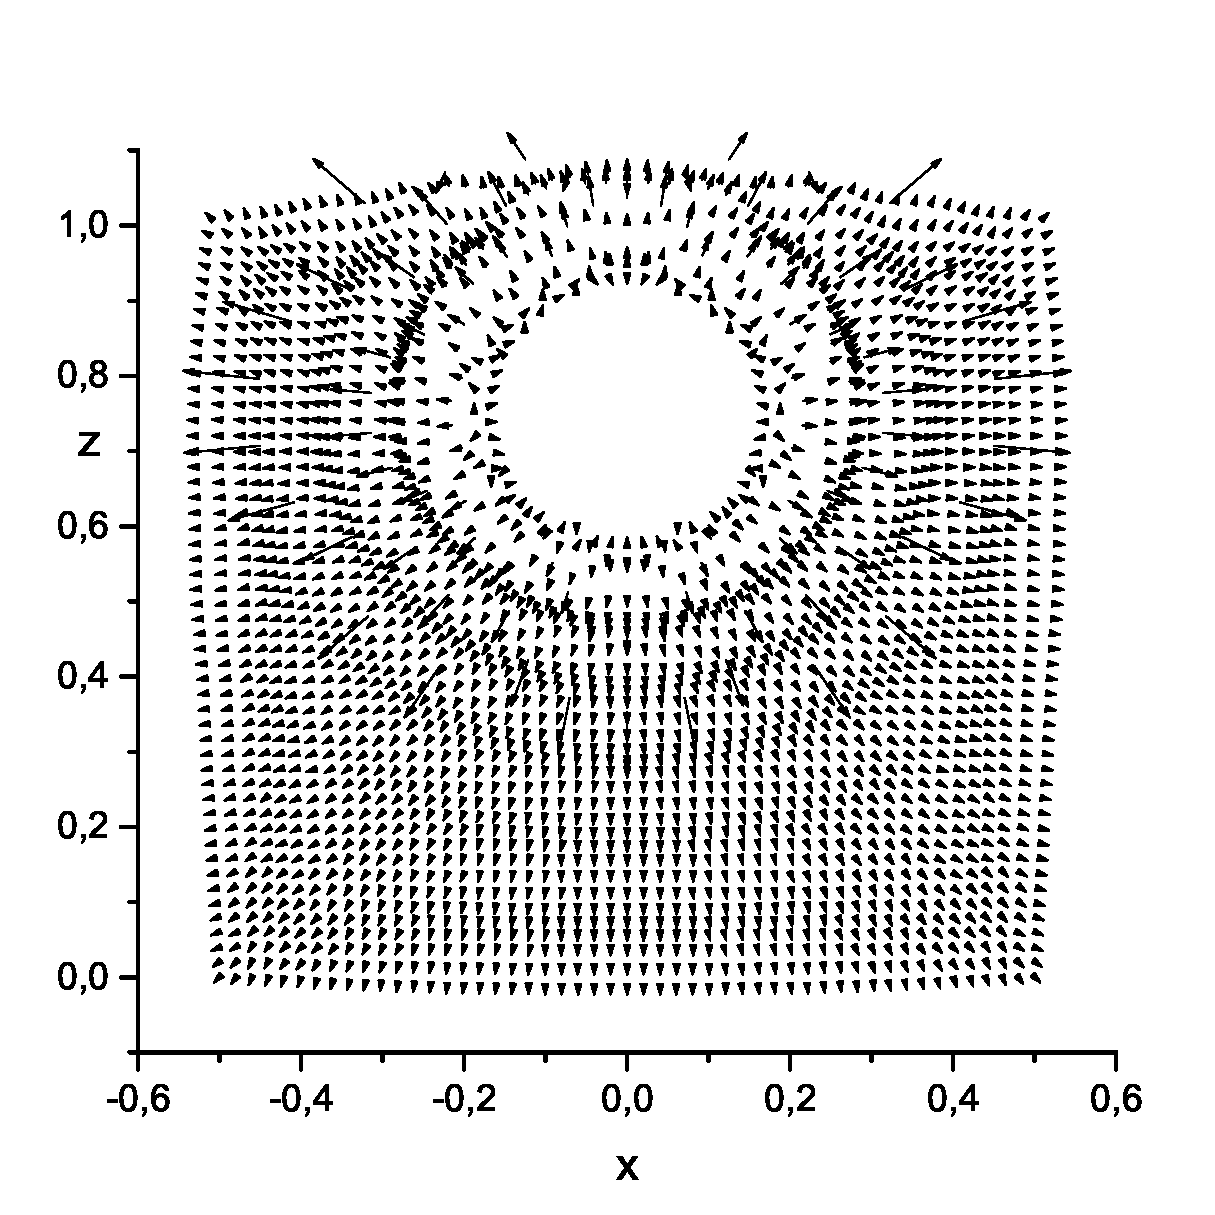
\includegraphics[width=0.4\textwidth]{Vel-25.eps}
\end{center}
\caption{\label{P-Vel-25} Distribution of pressure and particle velocities in the central section of the cube ($25$~$\mu$s)}
\end{figure}


After a few tens of microseconds pressure field substantially relaxes, only individual particles have the pressure greater then $p_0$, and scored the particle velocity continues to scatter out of inertia, thereby simulating the fraction of the liquid (Fig.~\ref{P-Vel-25}). One clearly sees a deformation of the side and bottom faces of the cube. The particle size distribution shows that inside a cube formed low-density zones, which lead to the growth medium fracture into fragments.

\begin{figure}
\begin{center}
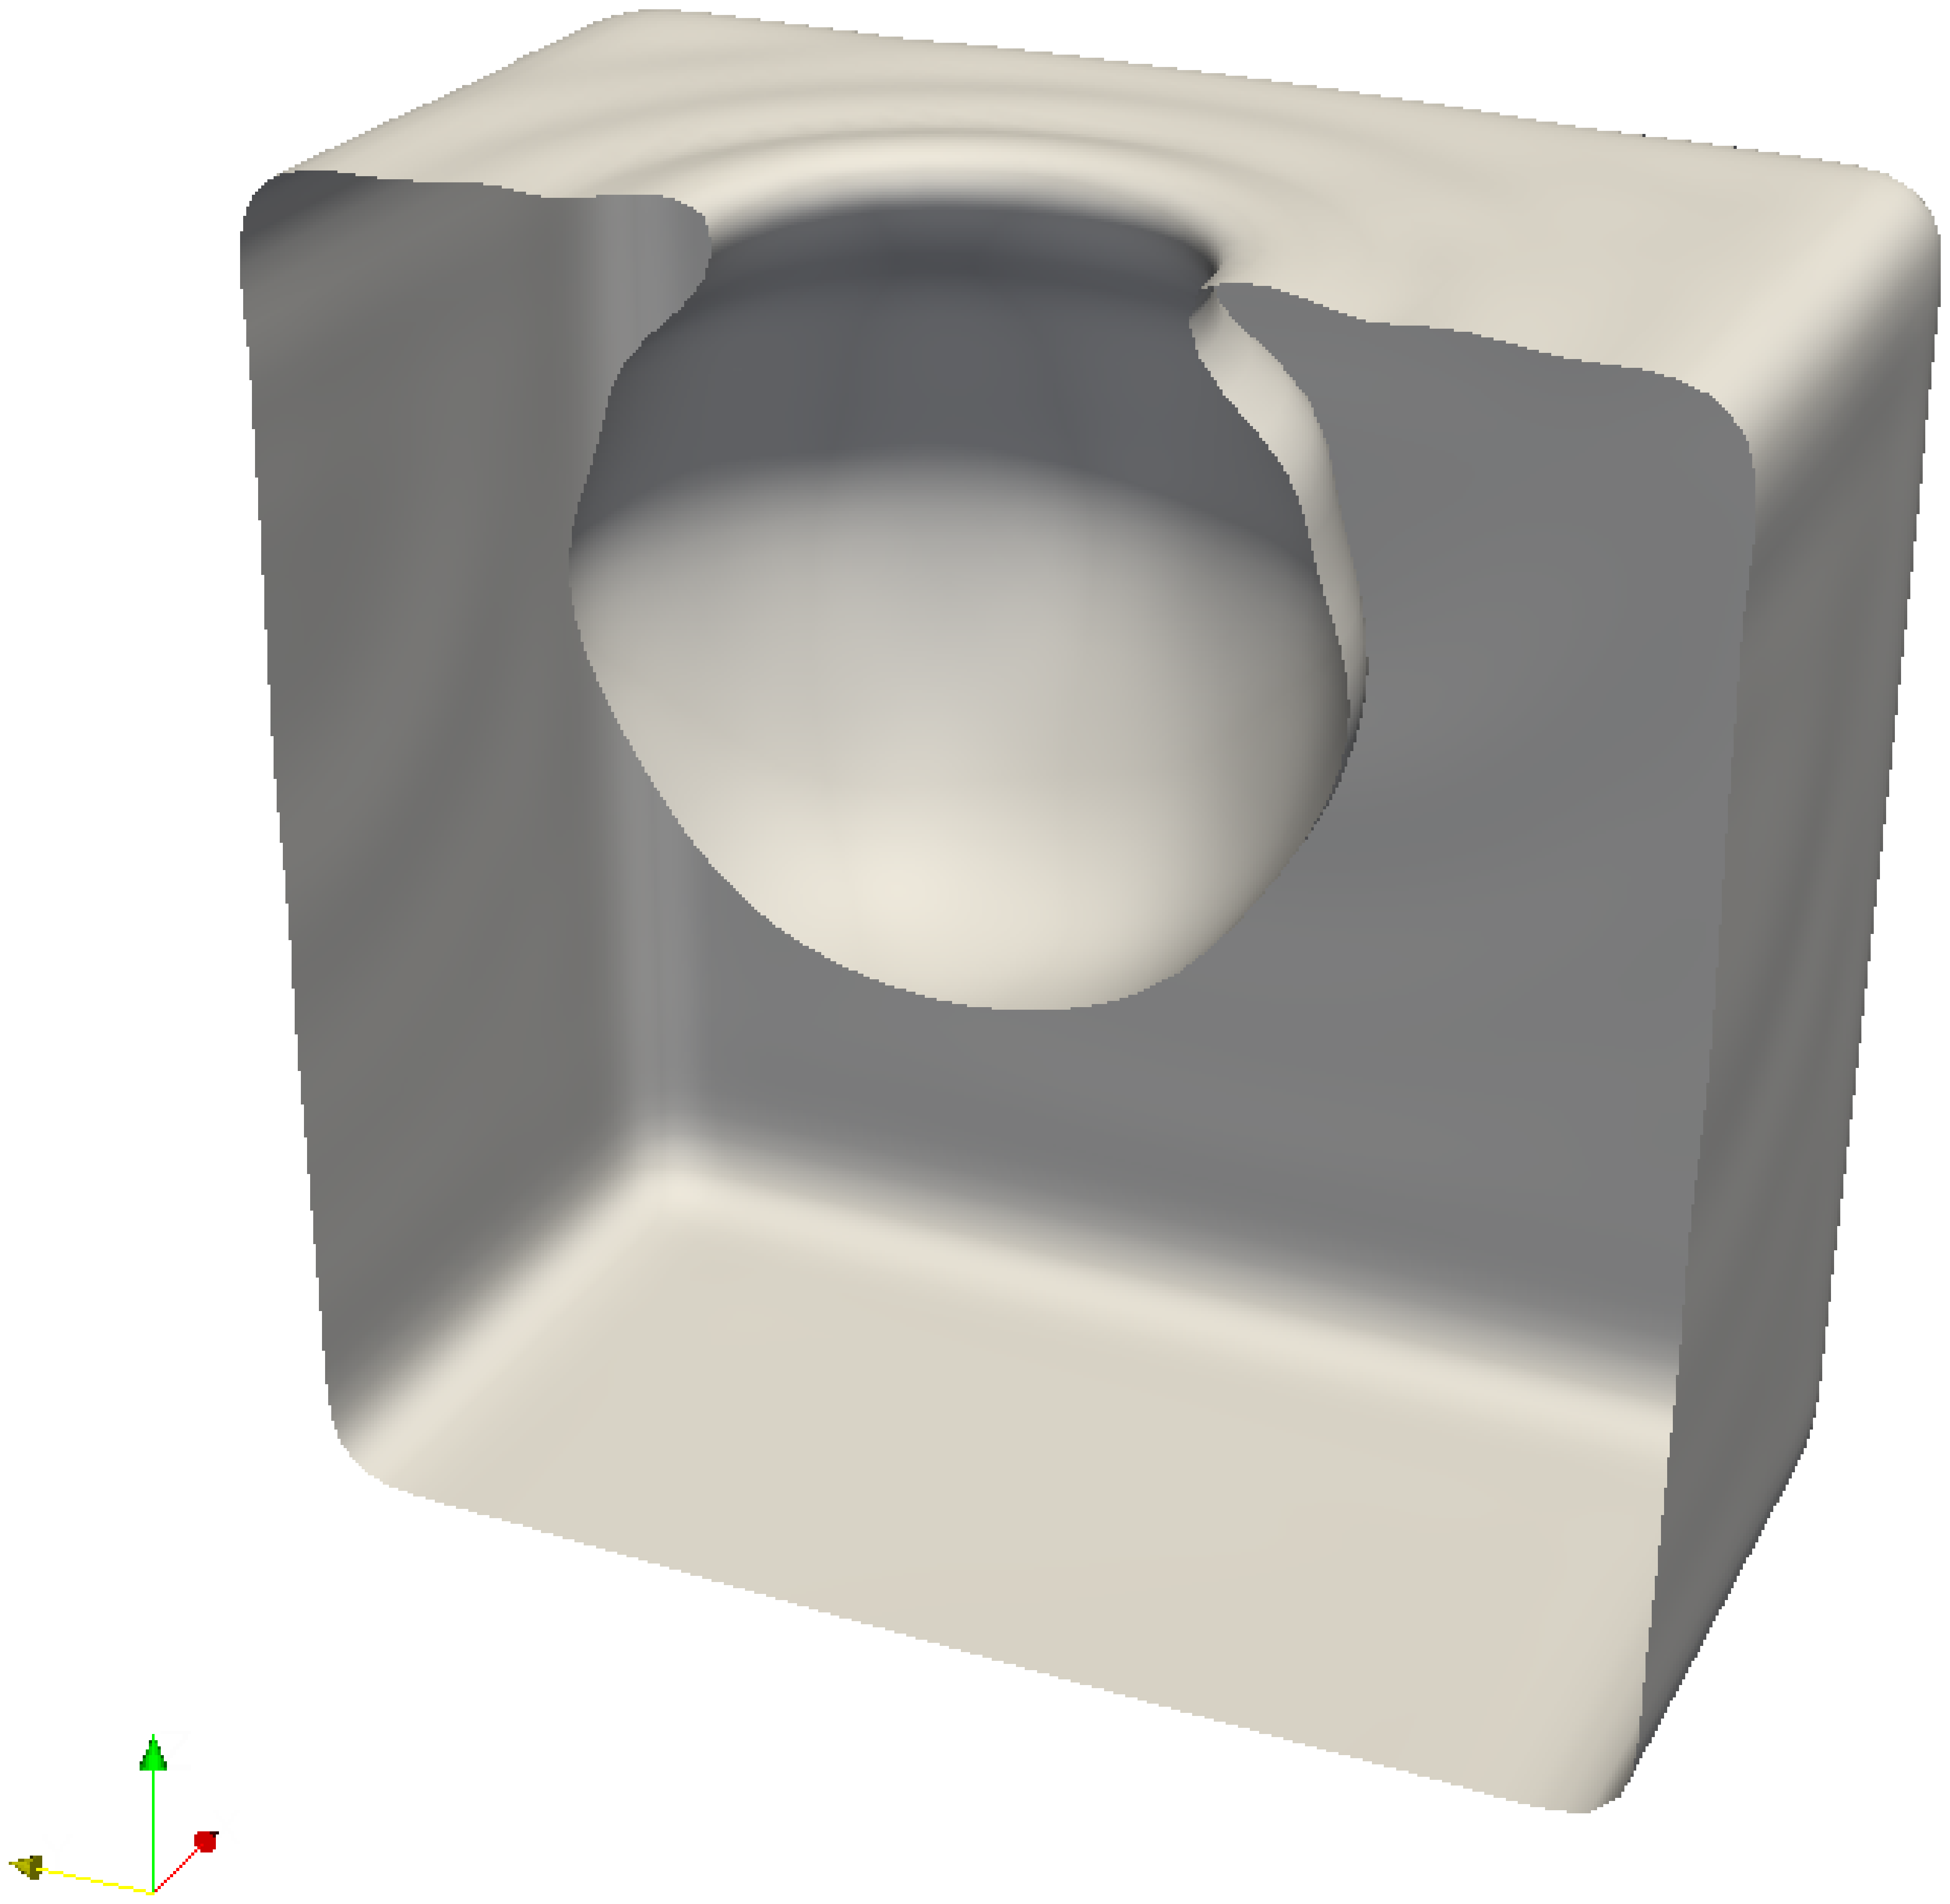
\includegraphics[width=0.4\textwidth]{3D-1.eps} \hfill 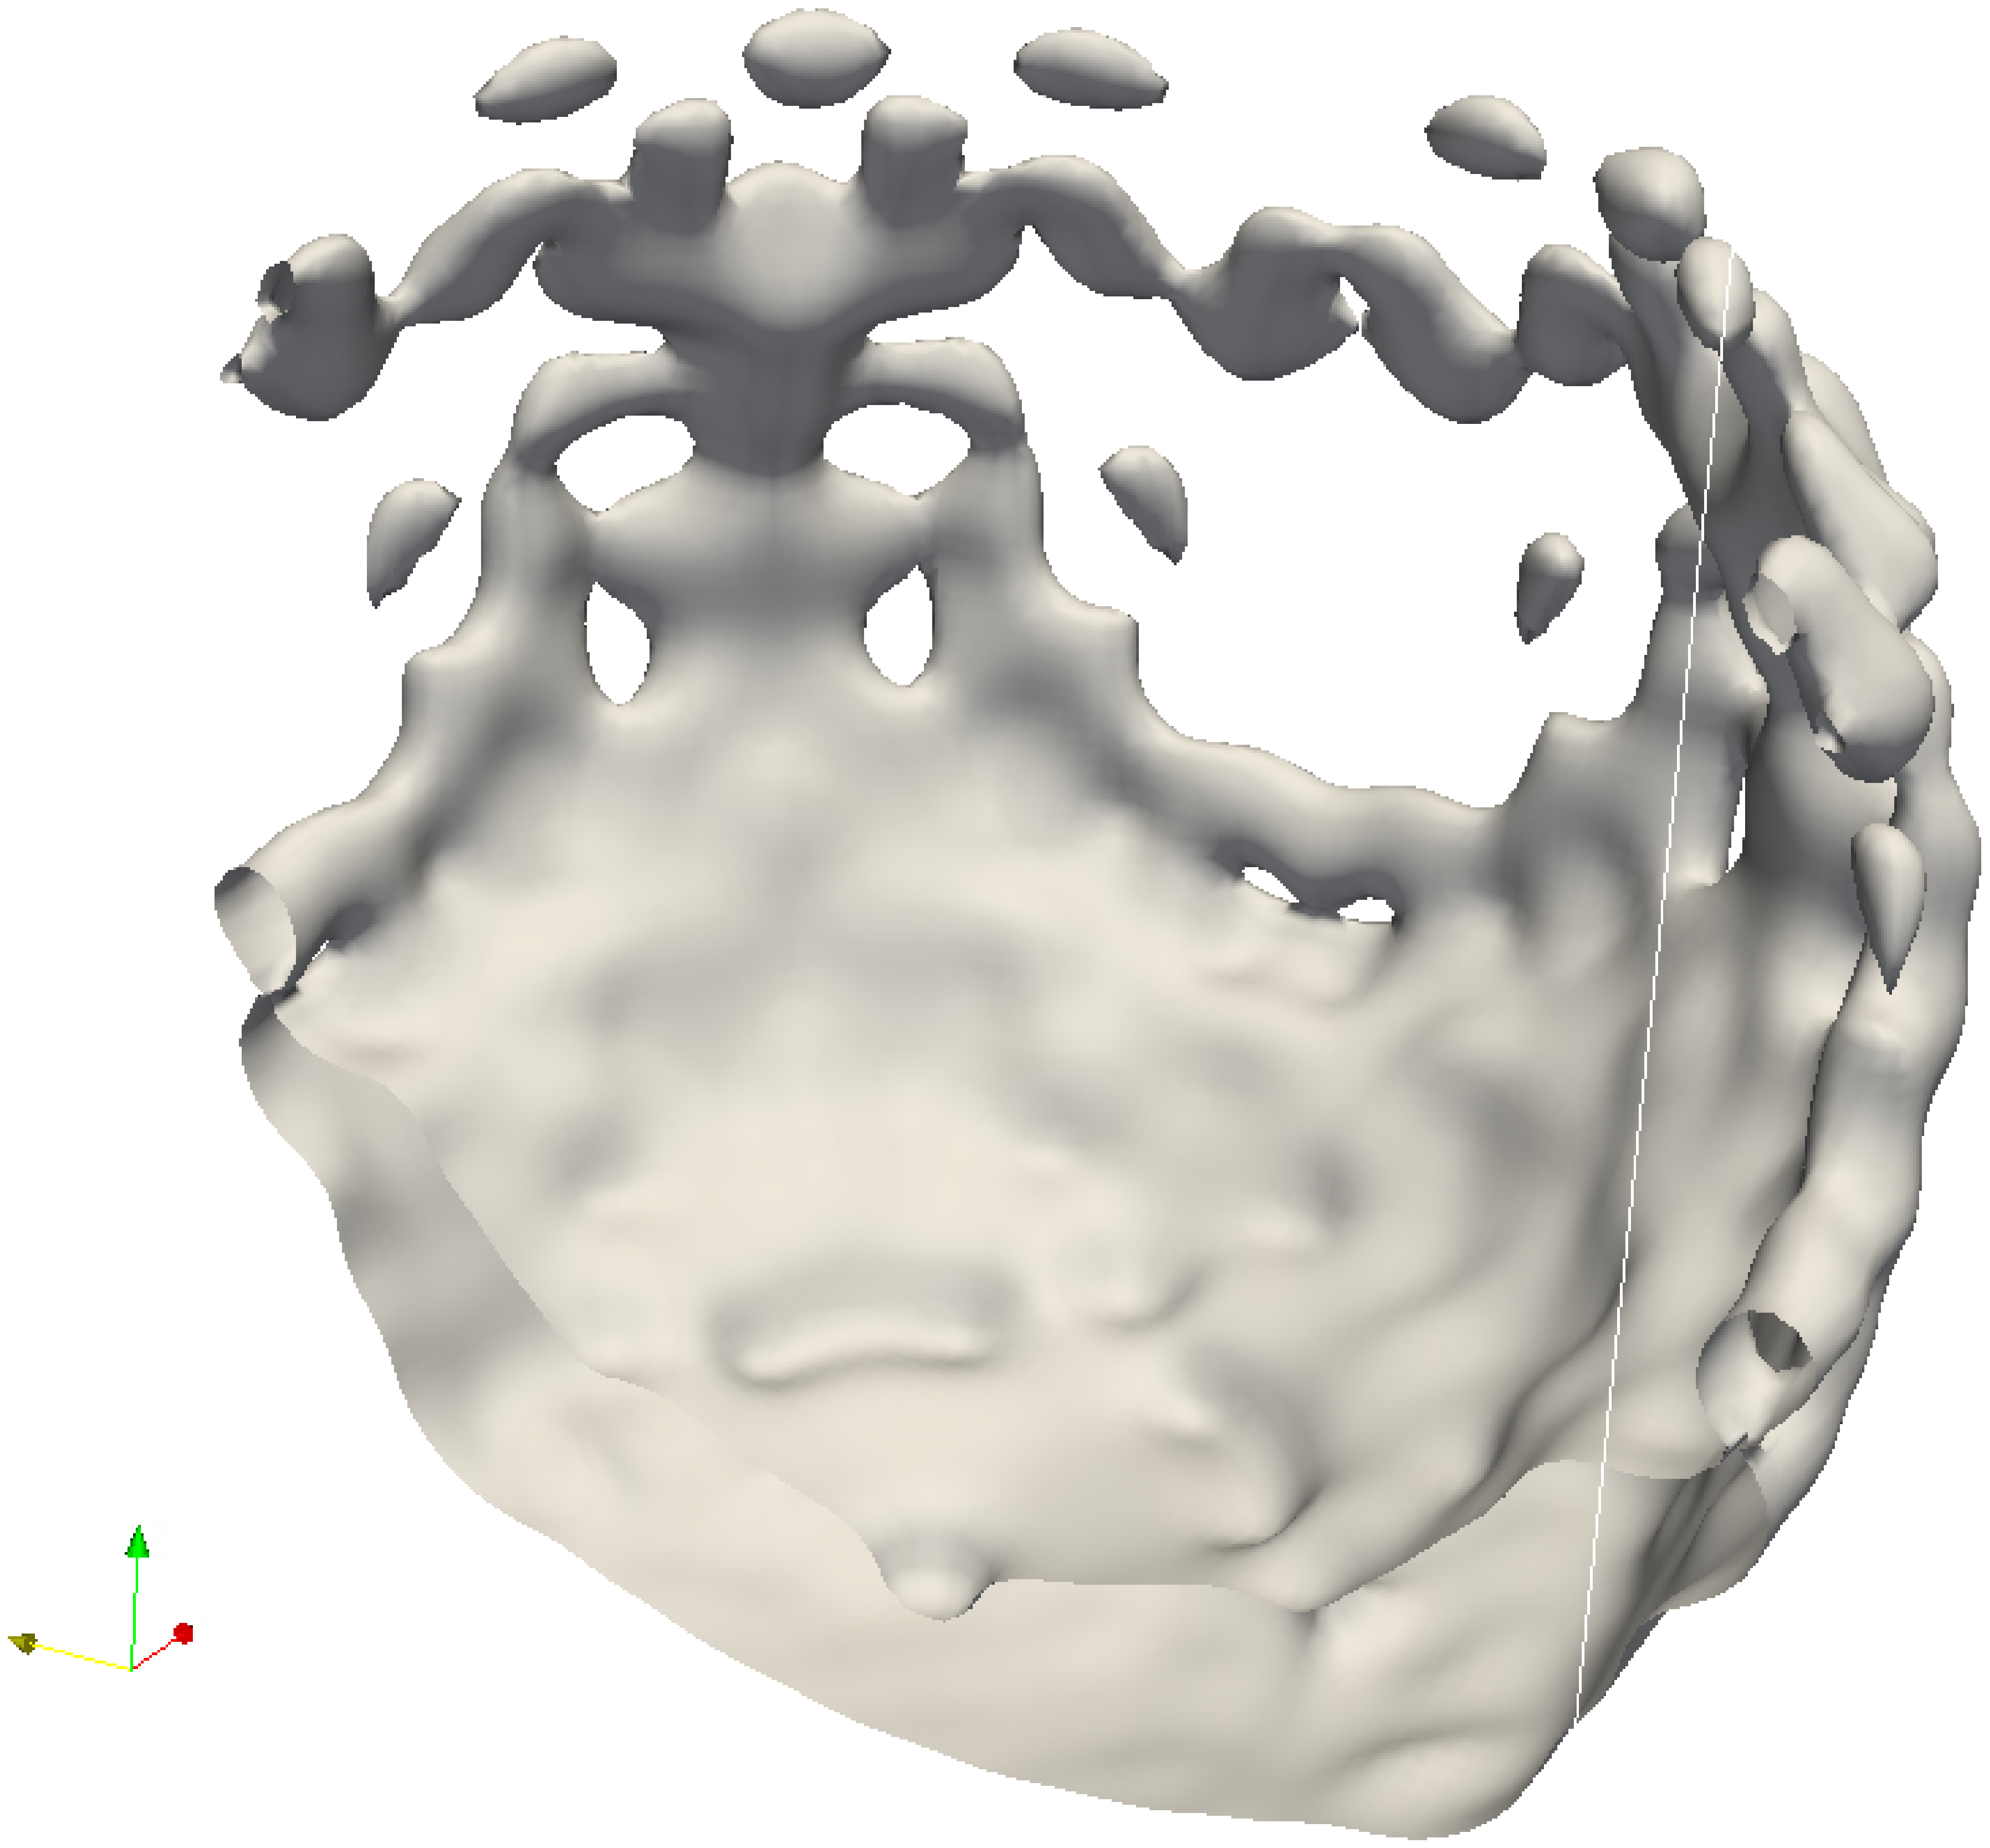
\includegraphics[width=0.4\textwidth]{3D-2.eps}
\end{center}
\caption{\label{3D-1} Isosurface $\rho=0.45$ g/cm$^3$ for the 
half cube in times $500$ and $10000$~$\mu$s}
\end{figure}

Figure~\ref{3D-1} shows 
the development of process in 3D view, it is an isosurface of the density field for the half of the cube, the value of the density is $\rho^* = 0.45$ g/cm$^3$. It means  that the isosurface bounds the area where the density of the liquid is greater than or equal to the $\rho^*$. Clearly that by the time $500$~$\mu$s (Fig.~\ref{3D-1}a) the cavity has increased in size by several times, ``stretched'' up and deformed the top face of the cube, the hole is formed. Bottom and side faces of the cube is slightly deformed. 


It should be noted that the same liquid particles spreads to distances greater than the smoothing radius, which means the loss of bonding in the SPH formulation and is interpreted as the medium fracture~\cite{DavydovKedrinskii2013}.

In the future, the vertical jet of liquid is formed on the top face of the cube, which gradually destroyed. Flying off individual spalls are formed on the side and bottom faces, where the destruction is not so strongly expressed (Fig.~\ref{3D-1}b).
In the future and in these areas the destruction of the liquid will occur and the emergence of a breakaway from the main volume of "layers". It is evident that the environment, flying away, loses consistency and disintegrates into fragments.
Further development of the process leads to the dissipation of the particles and the final destruction of the liquid.

\section{Conclusion}

The results of the numerical analysis of the processes of formation and dynamics of the structure of spalling zones after reflection of the shock wave generated by an underwater explosion from the free surface are presented. It shows that the SPH method can be used to study the dynamics of the liquid cube fracture.  A numerical simulation shows that the shock wave reflection from the free surface leads to relax of a high pressure and subsequent decomposition into individual fragments and clusters of almost free particles.

\ack{This work was supported by the
Russian Foundation for Basic Research (Grant No. 15-05-03336).}

\section*{References}
%\bibliographystyle{unsrt}
\bibliographystyle{iopart-num}
\bibliography{d:/Dropbox/BibtexBase/Work}


\end{document}